\section{Luồng active training data và train model}

Luồng này mô tả quy trình tận dụng dữ liệu phản hồi thực tế hoặc dữ liệu được quản trị viên chuẩn hóa để bổ sung vào tập huấn luyện, sau đó kích hoạt huấn luyện mô hình mới. Đây là chu trình cải tiến liên tục, giúp chatbot thích nghi với câu hỏi mới và nâng độ chính xác của phân loại intent cũng như điều phối hội thoại.

\begin{figure}[H]
    \centering
    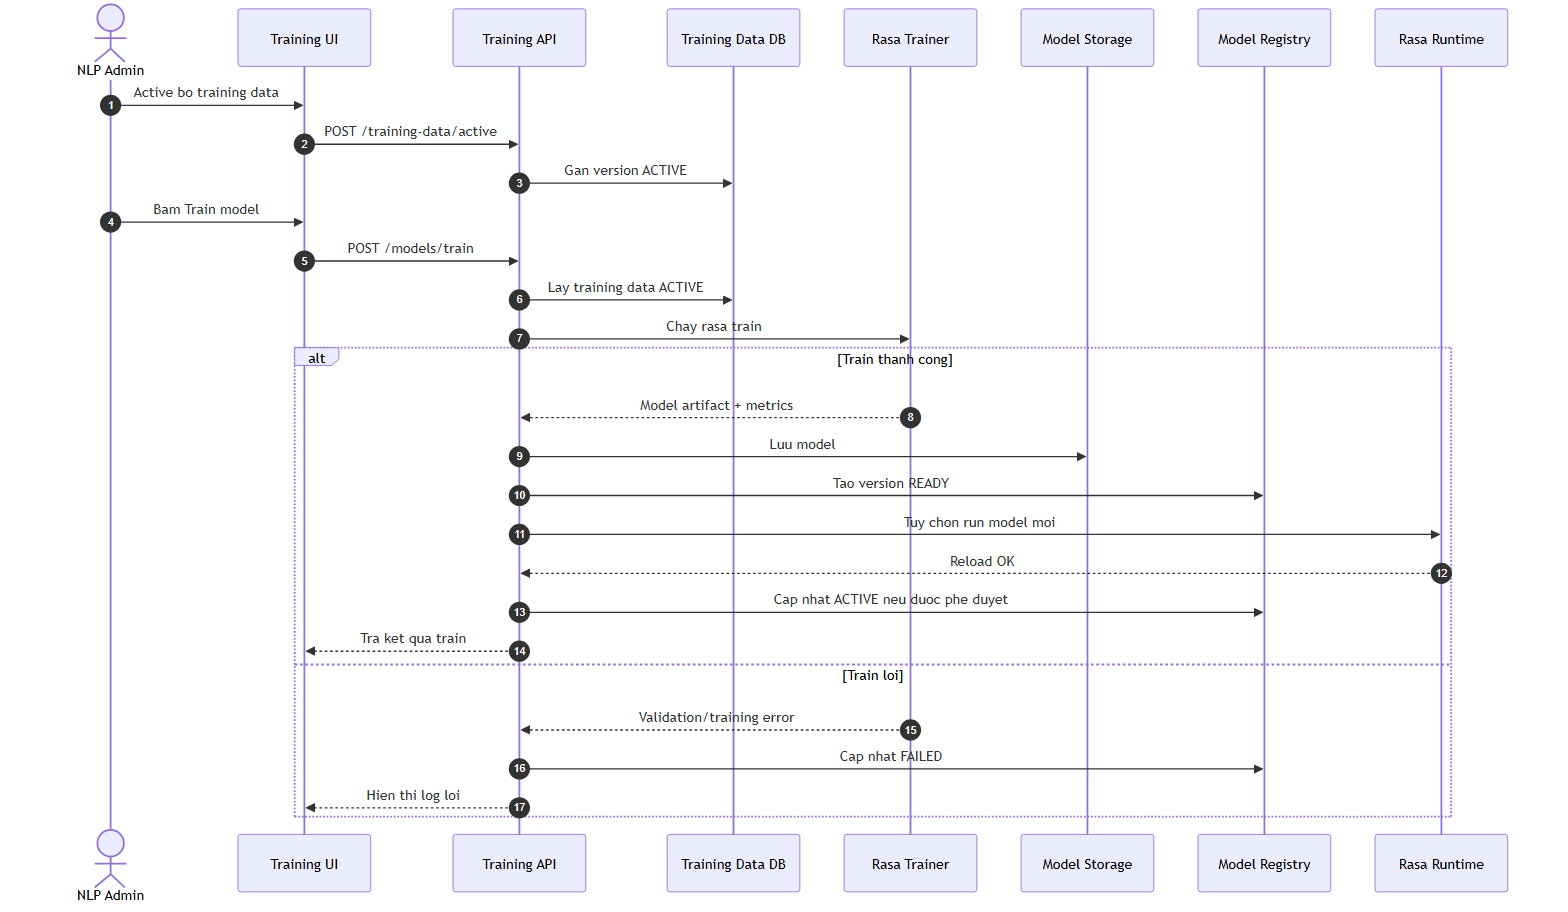
\includegraphics[width=\textwidth]{content/source/mermaid_sequence/seq_06.png}
    \caption{Luồng active training data và train model}
\end{figure}

Về nghiệp vụ, dữ liệu huấn luyện được duyệt hoặc chọn từ giao diện quản trị, chuyển tới backend để tổng hợp cùng intent, entity, rule và story hiện hành, sau đó hệ thống gọi tiến trình train model. Khi quá trình train hoàn tất, metadata về mô hình mới được lưu lại và giao diện có thể tiếp tục sử dụng luồng upload/run model để đưa mô hình vào vận hành. Sequence này thể hiện rõ chu trình dữ liệu từ quan sát thực tế đến cải tiến mô hình.
